\documentclass[11pt]{article}

\usepackage{hyperref}
\usepackage{xcolor}
\usepackage{calc}
\usepackage{graphicx}
\usepackage{tikz}
\usepackage{fontspec}
\usepackage{fontawesome5}
\usepackage{titlesec}
\usepackage{enumitem}
\usepackage{fancybox}
\usepackage{ctex}
\usepackage{multicol}

\hypersetup{hidelinks}

%%%%%%%%%%%%%%%%%%%%
% 设置
%%%%%%%%%%%%%%%%%%%%

% 本简历是基于 https://www.overleaf.com/latex/templates/seu-cv-dong-nan-da-xue-latex-zhong-wen-jian-li-mo-ban/jyzpthvnbmpm
% 修改的,最早的来源应该是 https://www.overleaf.com/latex/templates/npu-cv/mncqzxhvfzrx
% 恰好,我同最早的这位作者认识

% 本简历是在 VSCode 上编译的,记得采用 lualatex 或者 xelatex 编译
% vscode 可在左端 TEX 这一栏 的 Build 里面找到这两种 recipe
% 由于作者学艺不精也没太多时间,只是自己需要顺便做了一下,可能使用起来还需要调整
% 最顶上的花纹和最下面的花纹都是作者重新用PS做的,分别是 Riemann 曲面和 Calabi-Yau 流形


\definecolor{primary_color}{RGB}{42, 124, 116}    % 上师大青
\definecolor{secondary_color}{RGB}{245,76,0}  % 数理红



\setlength{\parindent}{0pt}					% 取消全局段落缩进
\pagenumbering{gobble}						% 取消页码显示
\setlist[itemize]{nosep                     % 取消 itemize 的默认间距
    , before={\vspace*{-\parskip}}          % 取消 itemize 和后续段落之间的空白
    , leftmargin=*}		                    % 取消 itemize 的左边距
\setlist[enumerate]{leftmargin=*}	        % 取消 enumerate 的左边距
\renewcommand{\arraystretch}{1.2}           % 设置表格行间距
\linespread{1.25}                           % 设置正文行间距

% 修改线条粗细


\titleformat{\section}					    % 将原标题前面的数字取消了
  {\LARGE\bfseries\raggedright} 		      % 字体改为 LARGE,bold,左对齐
  {}{0em}                      			  % 可用于添加全局标题前缀
  {}                           			  % 可用于添加代码
  [{\color{secondary_color}\titlerule}]     % 标题下方加一条线
\titlespacing*{\section}{0cm}{*1.2}{*1.2}	% 标题左边留白,上方,下方

\usepackage[
	a4paper,
	left=1.2cm,
	right=1.2cm,
	top=1.5cm,
	bottom=1cm,
	nohead
]{geometry}                                 % 页面边距设置

% 字体设置
\setmainfont[
    Path=fonts/,
    Extension=.otf,
    BoldFont=*-Bold,
]{NotoSerifSC}



\newlength{\iconwidth}
\setlength{\iconwidth}{1.5em}                   % 设置 section 标题部分图标占用的宽度

%%%%%%%%%%%%%%%%%%%%
% 文章内容
%%%%%%%%%%%%%%%%%%%%

% 学院
\newcommand{\school}{数理学院 | Mathematics \& Science Colledge} 

% 联系方式
\newcommand{\contact}{
    % 根据个人喜好选择字号
    % \small                % 小
    \footnotesize           % 更小
    % \scriptsize           % 再小一号
    \textcolor{white}{
        % 邮箱
        \faEnvelope \quad \href{mailto:123456@shnu.edu.cn}youremail@smail.shnu.edu.cn
        \hspace{4em}
        % 手机号
        \faPhone \quad  1xxxxxxxx
        % 别的联系方式,如微信、GitHub等
        \hspace{4em}
        \faGithub \quad \href{https://github.com/ZZH-DSL/}{ZZH-DSL}
        % 这个项目的地址
    }
}

\begin{document}

    %%%%%%%%%%%%%%%%%%%%
    % 页眉、页脚和背景(如果有多页简历,请把页眉页脚和背景复制粘贴到第二页的内容之前)
    %%%%%%%%%%%%%%%%%%%%

    % 页眉:校标组合+学院名
    \begin{tikzpicture}[remember picture, overlay]
        \node[anchor=north, inner sep=0pt](header) at (current page.north){
            
\includegraphics[width=\paperwidth]{header-darkgreen.png}
        };
        \node[anchor=west](school_logo) at (header.west){
            \hspace{0.5cm}
            
\includegraphics[width=0.2\textwidth]{banner-white.png}
        };
        \node[anchor=east](school_name) at(header.east){
            \textcolor{white}{\textbf{\school}}
            \hspace{0.5cm}
        };
    \end{tikzpicture}
    \vspace{-3.5em}

    % 页脚,联系方式
    \begin{tikzpicture}[remember picture, overlay]
        \node[anchor=south, inner sep=0pt](footer) at (current page.south){
            
\includegraphics[width=\paperwidth]{footer-darkgreen.png}
        };
        % 联系方式
        \node[anchor=center] at(footer.center){\contact};
    \end{tikzpicture}

    % 背景
    \begin{tikzpicture}[remember picture, overlay]
        \node[opacity=0.05] at(current page.center){
            
\includegraphics[width=0.7\paperwidth, keepaspectratio]{shnu.png}
        };
    \end{tikzpicture}

    %%%%%%%%%%%%%%%%%%%%
    % 简历正文
    %%%%%%%%%%%%%%%%%%%%

    \begin{minipage}[t]{0.78\textwidth}
        % 个人信息
        %  \fa 开头的是 {fontawesome5} 包里的,可以上网搜索各类图标
        \begin{minipage}[t]{\textwidth}
        \section[个人信息]{\makebox[\iconwidth][c]
        {\color{primary_color}{\faAddressCard}}\quad 个人信息}
        \begin{minipage}[t]{0.5\textwidth}
            \textbf{姓\qquad 名}: 伽罗瓦
            
            \vspace{0.5em}
            \textbf{出生年月}: 1811
        \end{minipage}
        \begin{minipage}[t]{0.35\textwidth}
            \textbf{性\qquad 别}: 决斗之神
            
            \vspace{0.5em}
            \textbf{政治面貌}: 一般路过法国民众
        \end{minipage}
        \vspace{1.2em}
        \end{minipage}

        % 教育背景
        \begin{minipage}[t]{\textwidth}
        \section[教育背景]{\makebox[\iconwidth][c]{\color{primary_color}{\faGraduationCap}}\quad 教育背景}
        
        {\large \textbf{法国高等师范学院}}, 专科 \hfill 2018年9月--2022年6月
        
        \vspace{0.5em}
        {\large \textbf{上海师范大学}}, 本科 \hfill 2022年9月--2026年6月
        \begin{itemize}
            \item 数理学院, 数学与应用数学 
            \item \textbf{主修课程}: 数学分析、高等代数\ 等. 
            \item \textbf{GPA}: 4.01 / 4.00 (排名: 1 / 10000) 
            \item \textbf{英语水平:} \textbf{CET4:} 750 \qquad \textbf{CET6:} 1000 % 可以再加雅思托福
        \end{itemize}        
        \vspace{1.2em}
        \end{minipage}
    \end{minipage}
    \hfill
    % 右半边,照片,比例占行宽20%
    \begin{minipage}[t]{0.2\textwidth}
        \vspace{2em} % 照片上侧内容
        \setlength{\fboxsep}{0pt}
        \fbox{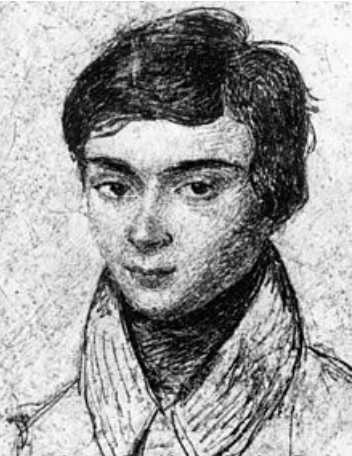
\includegraphics[width=0.8\linewidth]{150_200.png}}% 记得改为你自己的照片
    \end{minipage}
    
    \begin{minipage}[t]{\textwidth}
    \section[学科竞赛]{\makebox[\iconwidth][c]{\color{primary_color}{\faAtom}}\quad 学科竞赛}
         \begin{tabular}{l c c c c}
             \textbf{第xx届全国大学生数学竞赛 (数学 A 类)} &  &  & x等奖 & 20xx年xx月 \\
             \textbf{20xx年全国大学生数学建模竞赛} & x人队伍 & 建模/代码/论文& 四等奖 & 20xx年xx月\\
             \textbf{美国大学生数学竞赛} & x人队伍 & 建模/代码/论文 & P奖 & 20xx年xx月\\
             % 同理,可以自己加
         \end{tabular}
     \end{minipage}

    \begin{minipage}[t]{\textwidth}
    \section[实践经历]{\makebox[\iconwidth][c]{\color{primary_color}{\faChalkboardTeacher}}\quad 实践经历}
    
    \vspace{0.5em}
    {\large \textbf{HEO 代数几何讨论班}}, 主讲 \hfill 20xx 年 x 月
    \begin{itemize}
        \item \textbf{主要内容}: 导出范畴, Weil 猜想\ 等。
    \end{itemize}

    \vspace{0.5em}
    {\large \textbf{教师实习}}, TSU \hfill 20xx-20x 学年第x学期
    \begin{itemize}
        \item \textbf{主要内容}: 激情献唱 Only Yau \ 等。
    \end{itemize}

    \vspace{0.5em}
    {\large \textbf{累计志愿服务时长 xx 小时}}, 志愿干饭, 志愿打瓦等. 

    % 如果你有论文也可以修改一下标题展示论文,但我劝你不是正儿八经的数学论文别有
    
    \vspace{1.2em}
    \end{minipage}

    \begin{minipage}[t]{\textwidth}
    %所获荣誉
    \section[所获荣誉]{\makebox[\widthof{\faStar}][c]{\color{primary_color}{\faStar}}\quad 所获荣誉}
     \begin{multicols}{2}
         \begin{itemize}
             \item 20xx-20xx 国家级奖学金
             \item 20xx-20xx 专业x等奖学金
         \end{itemize}

         \begin{itemize}
            \item 睡觉大王
            \item 计算出了实对称矩阵的复特征值重大发现奖
         \end{itemize}
     \end{multicols}
     \vspace{1.2em}
    \end{minipage}
    
    
    % 如果每行的内容不是很多,可以考虑使用 minipage,将内容分列展示
    \begin{minipage}[t]{0.6\textwidth}
        \section[个人总结/自我评价]{\makebox[\iconwidth][c]{\color{primary_color}{\faAndroid}}\quad 个人总结/自我评价}
        \begin{itemize}
        \setlength{\itemsep}{0.5em}
            \item 我数学学得不错, Cauchy 都说好. 
            \item 我枪法不错. 
            \item 我的论文浓缩法强于 Gauss. 
            \item 谢谢你 Liouville. 
        \end{itemize}
    \end{minipage}
    \hfill
    \begin{minipage}[t]{0.35\textwidth}
        \section[兴趣爱好]{\makebox[\iconwidth][c]{\color{primary_color}{\faStar}}\quad 兴趣爱好}
        \begin{itemize}
        \setlength{\itemsep}{0.5em}
            \item 数学
            \item 恋爱
        \end{itemize}
    \end{minipage}
    
    % \newpage
    % % 如有需要,可以添加额外的页面。不要忘记添加页眉页脚和背景相关的代码。

    % % 技能特长
    % \section{\makebox[\widthof{\faWrench}][c]{\color{primary_color}{\faWrench}}\quad 技能特长}
    % \begin{itemize}
    %     \item 熟练使用\Cpp 、Python、Matlab编程语言。
    %     \item 熟悉Windows与Linux端开发。
    %     \item 熟练使用Tensorflow,Pytorch等深度学习框架。
    %     \item 熟练掌握\Cpp 与Python环境下OpenCV与Qt应用的开发,且熟练使用Qt Creator软件。
    %     \item 熟练使用Altium Designer与LCEDA进行封装绘制与板子设计。
    %     \item 熟练使用Keil,Arduino IDE等集成开发软件。
    %     \item 了解模式识别,强化学习,遗传算法,知识蒸馏等相关概念。
    % \end{itemize}

    % % 其他
    % \section{\makebox[\widthof{\faInfo}][c]{\color{primary_color}{\faInfo}}\quad 其他}
    % \begin{itemize}
    %     \item 英语水平-CET6级xxx分
    %     \item 计算机几级证书
    %     \item xx几级证书
    %     \item 技术博客: 某网址
    %     \item 教师资格证:xxx
    %     \item 普通话证书:几级几等
    %     \item 文字排版:\LaTeX
    % \end{itemize}

\end{document}
